\section{绪论}
\zihao{-4}
\setlength{\baselineskip}{20pt}
\fancyhf{}
\renewcommand{\headrulewidth}{0.5pt}
\fancyhead[C]{\zihao{-5}基于MaskedFaceNet的智慧工厂管理系统}
\fancyfoot[C]{\zihao{-5}\tnr\thepage}
\pagenumbering{arabic}

\subsection{研究背景}

随着信息技术的高速发展,越来越多的行业领域开始与这一学科开始交叉挂钩,并且结合出了非常多样的理论知识与应用场景。关于信息管理系统,不管各行各业,无论是高校学籍档案、医疗设备信息还是农业大棚温度测控的场景,都离不开简单高效信息管理系统应用。而且在一些特定的应用场景,不同的信息管理系统所面向的功能也不尽相同,例如有些系统需要面对超大批量用户访问的高并发场景,而有些系统则需要在信息的安全性方面做进一步加强。然而在一些中小型企业工厂的信息管理方式中,例如对工厂员工的信息、客户信息、供应商信息、产品信息以及原材料信息的管理,工厂管理人员大部分往往都是通过手工的方式对信息进行管理,即使人们会用到一些办公软件,例如Word、Excel等;工厂与客户以及供应商的合作方式还都是以电话、微信等联系方式进行沟通交流,但这种方式毫无疑问是离散的、不统一的,并且信息的传递往往都并不是实时的,所以针对中小型工厂企业,设计实现一个通用的、简单易管理的信息管理系统往往有着很大的需求。

人脸识别(Face Recognition)作为一种主流生物识别技术,已经充分的渗透各个领域之中,例如军事、金融、公共安全和日常生活等。并且人脸识别在CVPR(Computer Vision and Pattern Recognition)社区一直是一个火热并且存在长久的研究话题。在上个世纪末,基于特征的人脸识别技术的里程碑出现了,通过特定的分布假设,派生出了一些综合的数学方法对数据的低维表示。直到二十一世纪初,一个众所周知的问题便是这些理论上似乎可信的综合数学方法无法处理的,那就是不可控的面部改变问题。这些问题在\cite{deepfrsurvey}中提到的人脸识别的四个关键时期中,前三个时期尽管解决人脸识别中的某些面部变化问题,例如姿势变化、光线亮度变化、面部表情和伪装打扮等,但是解决这些问题的方法往往都是比较单一,而且对于识别准确性的提升都是非常有限的。然而这一切都在2012年AlexNet使用了深度学习技术赢下了ImageNet图像分类竞赛的时候发生了巨大的改变。深度学习使用诸如卷积神经网络模型,将多层处理单元进行级联,对输入数据的特征进行提取和变换,从而得到输入数据的多层抽象表示。通过这些多层次的抽象表示,对于人脸姿势、面部表情和光照强度都有着非常强大的不变特性。并且人脸识别技术随着深度学习技术一同飞速发展,直到今天,各种各样的用于人脸识别系统中各个模块的网络模型,都有着超越人类表现的性能。

% \begin{figure}
%     \centering
%     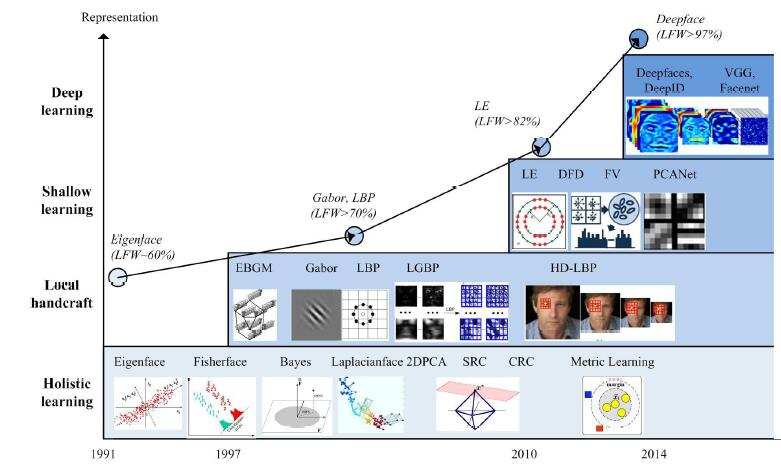
\includegraphics[width= \textwidth]{figures/1maintime.jpg}
%     \caption{人脸识别技术的四个关键时期}
%     \label{fig:maintime}
% \end{figure}

\subsection{国内外研究现状}

在2012年,随着AlexNet\cite{alexnet}在ImageNet图像分类的竞赛上以非常优越的性能超越了当时的所有模型的结果,人们开始考虑将用于图像分类的网络模型作为骨干结构来构造人脸识别系统,例如Deepface\cite{deepface}。到了2015年,由Google提出的一个22层的GoogleNet\cite{googlenet}网络模型,人们开始将网络模型变得越来越“深”,深度学习这一技术开始受的越来越多人们研究。同年,将GoogNet作为主干结构,Goole再次提出了一个网络模型Facenet\cite{facenet}用于构造人脸识别系统,该网络模型提出了一种名为TripletLoss的损失函数,此系统可以直接学习将输入的人脸图像映射到欧氏距离空间中,相同身份的图像有着更近的距离,不同身份的图像则有着更远的距离。Facenet将输入图像映射到一个128维的embedding空间中,用于比较不同人脸图像的相似度。该系统在Labeled Faces in the Wild(LFW)数据集上实现了$99.63\%$的准确率,在On YouTube Faces DB数据集上实现了$95.12\%$的准确率,在当时有着最先进的性能。

随着网络模型变得越来越深,很多大型的网络模型有着上百万的参数用来训练优化,人们发现以传统的损失函数作来对用于人脸识别网络模型的训练变得越来越难以收敛。所以,人们开始将研究重点放在各种训练技巧上,例如设计各式各样的损失函数用于改变训练方式并且加快收敛速度。上文提到的TripletLoss损失函数是作为基于欧氏距离的一种,另一种损失函数的类型则是基于角度和余弦边距的损失函数,不同于将人脸图像映射到欧式空间中,第二种损失函数用于将不同身份的人脸图像,即学到的特征,变得更加具有分辨性,也就是增加它们的角度或是余弦距离,作为第二种损失函数类型的代表是Arcface\cite{arcface}提出的一种带有额外角度边距的损失函数,基于此损失函数构造的人脸识别系统,也实现了最先进的识别性能。

随着越来越多的网络模型被提出,人脸识别的准确率也一步步上升。但是,通常实现最先进性能的模型,往往都是由互联网巨头提出的,例如Google、Facecbook等,他们用于训练网络模型的数据集都是私人的人脸数据集,所以这使得很多研究人员无法准确的复现他们所报道的性能,这给学术界的研究人员带来了很大的挑战。为了解决这一问题,CASIA-Webface\cite{webface}首次提出了广泛使用的公开人脸训练数据集,此数据集有10,575位收集自互联网的人物,共494,414张人脸图像。然而,CASIA-Webface数据集相对较小的数据量和人物数量并不能反映出深度学习的很多高级特性。所以,VGGFace2\cite{vggface2}数据集便被提出了。此数据集有大约三百三十一万人脸图像分为9131个类别,每一个类别代表了一位身份人物。可以毫不夸张的说,人脸数据集的发展过程在很大程度上引领了人脸识别研究的方向。一个足够大的数据集,包含不同的人脸姿势、光线强度、面部表情、不同种族、不同年龄以及性别等,可以使得网络模型有着非常强大的泛化能力。

\subsection{研究目的与意义}

由于新冠疫情在全国范围内的影响,这使得人们的生活方式发生了全面的改变。上班人员开始居家办公,学生也开始在家上网课;这对线下实体的一些销售实体行业产生了巨大的冲击,由于新冠疫情具有强烈传染性,关闭了一些公共场所的商业店铺,社会生产方面全面停止生产。在我国政府以及中国健委会的管理控制下,新冠疫情在我国及时得到了有效控制。尽管如此,人们的日常出行方式须佩戴医用外科口罩。在此期间,以往的生物识别的认证方式并无法有效的防止病毒的入侵,例如,一些场所的通行方式是通过触摸电子屏幕等物体进行生物识别认证,如果没有及时做好清洁消毒工作,若之后触摸到了眼睛、鼻子或嘴巴等身体部位,也使得非常大的几率感染新冠病毒。所以,很多的出行场所将认证方式改为人脸识别,可以实现零触摸的生物认证,然而,在疫情还没有得到完全消除的背景下,通常这些场所都是人口比较密集的公共场所,所以人们在通往关口的时候还要佩戴口罩来有效抵挡病毒的入侵,但是由于佩戴了口罩将人脸进行了遮挡,这使得一些人脸识别的系统出现了失效问题,例如识别准确率下降或无法识别等问题,这给人脸识别领域带来了很大的挑战。所以研究人员要开始探索新的网络架构、损失函数的设计或对人脸进行遮挡的训练测试数据集等,来处理佩戴口罩带来的人脸识别失效的问题。

并且尽管在应对新冠疫情的时候,已经有了一套完整且系统的控制处理方式,这也引起了很多的线下实体生产产业的反思,人们开始考虑将一些业务逻辑结合信息技术在互联网平台上进行业务交流以及信息管理等。特别是对于一些中小型的生产工厂,工厂管理人员对员工信息的管理、客户信息、订单、生产原材料和供应商信息等管理方式往往都还是以半手工半信息技术的方式对工厂进行管理。并且对于一些生产工厂,工厂的安防问题也有着很大的隐患,所以结合深度学习技术,整合一个全面系统的工厂管理平台,既可以实现佩戴口罩的人脸识别以及处理安防问题,例如生产员工是否正确穿戴安全帽、防护服等,可以有效的提升工厂企业的生产效率。

\subsection{研究内容}

使用Django框架开发一个智慧工厂管理站点,前端页面使用Bootstrap框架设计,将数据存储到PostgreSQL数据库,对交易记录、员工信息、客户信息、供应商、产品和原材料等信息进行管理。并且结合深度学习技术,在Facenet网络模型的预训练模型之上,基于CASIA-Webface人脸数据集使用MaskTheFace工具对数据集中的人脸进行检测,并且将模板中的口罩对人脸进行遮罩,将口罩“佩戴”到人脸图像中,构造一个由10,575位人物、494,414张模拟佩戴口罩的人脸图像数据集进行微调训练,将训练好的模型整合到工厂管理系统中,可以用来作为车间出入、员工考勤打卡功能。除此,构造目标检测网络模型,对生产车间的生产情况进行实时安防监测,在特定的生产环境中,若员工没有正确穿戴安全帽、防护服等,可以通过工厂系统进行提醒。